\documentclass{article}
\usepackage{fullpage}
\usepackage[portuguese]{babel}
\usepackage[utf8]{inputenc}
\usepackage[protrusion=true,expansion=true]{microtype}
\usepackage{graphicx}
\usepackage{siunitx}
\usepackage{url}
\usepackage{listings}

\graphicspath{ {imgs/} }

\author{Henrique Aires Silva \\RA: 169574 \\ Turma T}

\newcommand{\horrule}[1]{\rule{\linewidth}{#1}} 	% Horizontal rule

\title{
  \usefont{OT1}{bch}{b}{n}
  \normalfont \normalsize \textsc{FEEC - Faculdade de Engenharia Elétrica e de Computação} \\
  \normalfont \normalsize EA871 - Lab. de Programação Básica de Sistemas Digitais
  \horrule{0.5pt} \\[1.0cm]
  \LARGE \textbf{Relatório do Experimento 2\\Ferramentas de Desenvolvimento de Software} \\[1.0cm]
  \horrule{2pt} \\[0.1cm]
}

\author{
  \normalfont 								\normalsize
  Henrique Aires Silva\\ \normalfont \normalsize RA: 169574 - Turma T\\[-3pt]		\normalsize
  \today
}
\date{}

\begin{document}
\maketitle

\section{Introdução}
Uma das etapas mais importantes do desenvolvimento de softwares embarcados é a rotina de testes (debug) junto ao Hardware selecionado. Esta tarefa nem sempre é a mais trivial, dado que o microcontrolador em que se deseja executar o software quase sempre não é o mesmo no qual se desenvolve. Além disso, por ser um ambiente de muito baixo nível lógico no sentido de abstrações, é praticamente inviavel testar o software desejado analisando as transações entre registradores internos do microcontrolador e mudanças lógicas de seus pinos.

Para amenizar alguns deste problemas e tornar a tarefa de desenvolvimento de software embarcado mais simples e acessível, foram criados softwares chamados de \textbf{IDEs} (Integrated Development Environments - Ambientes de Desenvolvimento Unificado) que tem por premissa abstrair o acesso aos registradores e informações de baixo nível do microcontrolador de modo que uma pessoa com minimos conhecimentos técnicos na área consiga com pouco esforço testar e corrigir, se necessário, seu software, focando seu esforço no desenvolvimento do algoritmo.

O IDE utilizado no curso de EA869 é conhecido como \textbf{CodeWarrior}\cite{code-warrior}, desenvolvido e mantido pela NXP (antiga Freescale). Nele estão presentes ferramentas de gerenciamento de projetos de software, editor de código, compilador e debugger, tudo em um mesmo ambiente.

Esta ferramenta é capaz de interfacear com o hardware da placa \textbf{FRDM-KL25}\cite{manual-frdm}, que possui como componente principal o microcontrolador \textbf{MKL25Z128}\cite{manual-mic}, além de diversos periféricos, como converso USB-Serial, sensor capacitivo de toque, diversos pinos de propósito geral (GPIO) e um LED RGB, que será o foco deste experimento.

\section{Objetivo}

Durante este experimento, procurou-se a familiarização do aluno com a ferramenta de desenvolvimento de software embarcado CodeWarrior.

Para alcançar tal objetivo, foi proposto que fosse criado um simples programa que controle um LED RGB e pisque na cor branca (todas as cores acesas) em um intervalo de tempo fixo.

Com o objetivo de  estimular boas práticas de programação e incentivar o reuso de código, foi proposto que fosse desenvolvido um código modular, ou seja, com arquivos separados por função objetivo, de tal modo que este possa ser utilizado em outros projetos da disciplina no futuro caso necessário.

\section{Metodologia}
\subsection{LED RGB}
O LED RGB é composto por 3 LEDs de cores distintas (Azul, Verde e Vermelho) no mesmo encapsulamento com um anodo comum como mostrado na Figura \ref{led_rgb}. Desta forma é possível acioná-los independentemente controlando o nível de tensão em seu catodo.
Por estarem no mesmo encapsulamento é possível gerar diversas combinações de cores acionando os LEDs em conjunto, dado que sua luz emitida será difundida e misturada.

\begin{figure}[ht!]
\centering

\includegraphics[width=70mm]{rgb_led.png}
\caption{Esquema elétrico de um LED RGB com anodo comum \label{led_rgb}}
\end{figure}

No escopo deste experimento, não será explorado o conceito de modulação de pulso, que pode ser utilizado para gerar diversos tons de cores com apenas as 3 cores primárias, apenas o acionamento lógico (ligado ou desligado) dos catodos. Assim, temos um total de 7 cores distintas possíveis.

Para gerar uma luz branca por exemplo, é possível acionar todos os 3 LEDs.

\begin{figure}[ht!]
\centering
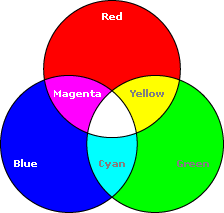
\includegraphics[width=40mm]{rgb_colors.png}
\caption{Diagrama mostrando as possíveis combinações de cores sólidas de um LED RGB \label{rgb_colors}}
\end{figure}

\subsubsection{Acionamento do LED RGB}

A conexão elétrica do LED RGB de anodo comum na placa MLK25Z128 segue um padrão bem conhecido, onde tem o pino comum ligado na alimentação positiva, e cada anodo sendo ligado em um pino independente do microcontrolador, com um resistor em série para limitar a corrente.

Este esquema é particularmente proveitoso pois ele contorna uma das dificuldades de todos os microcontroladores da atualidade, que é a capacidade baixa de fornecimento de corrente direto em pinos lógicos. Ou seja, se ligássemos o LED com o anodo ligado no pino lógico e o catodo no GND, dependendo do valor do resistor limitador, o controlador não conseguiria fornecer corrente suficiente para fazer o LED brilhar.

\begin{figure}[ht!]
\centering
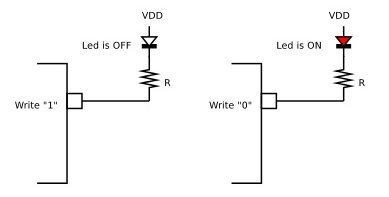
\includegraphics[width=85mm]{led_connect_sink.png}
\caption{Esquemático de uma ligação de um LED em um controlador usando lógica invertida \label{led_sink}}
\end{figure}


Por outro lado, os pinos lógicos tem uma grande capacidade de absorção de corrente, por conta de sua construção interna. Assim, podemos fazer a ligação mostrada na figura \ref{led_sink}

Desta forma, teremos uma lógica invertida no software, ou seja, para acionar o LED devemos escrever o nível lógico ''0'' no pino correspondente. Analogamente, para apagar o LED, basta escrever ''1'' em seu pino.

\subsection{Atrasos}

Como microcontroladores possuem períodos de relógio extremamente rápidos, da ordem de dezenas de nanosegundos, estes executam seus algoritmos de maneira quase imperceptível aos humanos.

Para que consigamos interpretar e interagir com o hardware, de forma a percebemos eventuais problemas, devemos fazer com o microcontrolador execute funções de atraso entre certos comandos que tem por objetivo a percepção humana, como o acionamento de um LED ou escrita de uma mensagem em um display.

Tais rotinas apenas fazem com que o processador fique parado num laço finito por um determinado tempo, sem realizar mais nenhum comando (não entram no escopo deste experimento as interrupções assíncronas), assim é possível que uma pessoa distingua o piscar de um LED por exemplo.


\section{Proposta de Solução}

Para implementar o software que pisca um LED RGB na cor branca, é necessário realizar uma série de inicializações e configurações do hardware, dado que após o Reset, o microcontrolador não tem como saber em que estado o hardware se encontra.

Neste desenvolvimento foi necessário utilizar funções apenas do módulo \textbf{GPIO} do controlador, dado que é apenas necessário alterar o nível lógico dos pinos conectados ao LED.

\subsection{Inicialização}
Visando a redução do consumo de energia do microcontolador, este foi fabricado de tal forma que fosse possível desabilitar o sinal de clock para cada módulo que não estivesse em uso. Este controle é feito através do conjunto de registradores \textbf{SIM\_SCGC} (\textbf{S}ystem \textbf{I}ntegration \textbf{M}odule - \textbf{S}ystem \textbf{C}lock \textbf{G}ating \textbf{C}ontrol).

Assim, após o ínicio do programa, precisamos habilitar o clock para o periférico \textbf{GPBIO\_B} e \textbf{GPBIO\_D} setando, respectivamente, os bits 10 e 12 através do registrador \textbf{SIM\_SCGC5}, como mostrado na figura \ref{sim_scgc5}.

\begin{figure}[ht!]
\centering
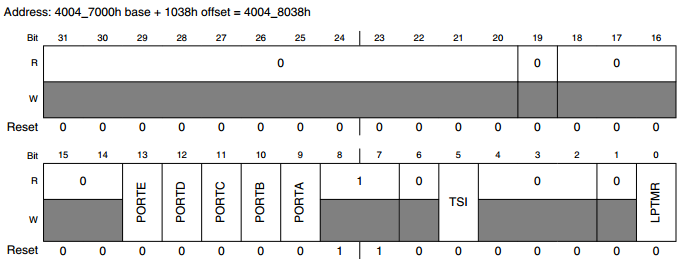
\includegraphics[width=100mm]{sim_scgc5.png}
\caption{Formatação do registrador SIM\_SCGC5, mostrando os bits de ativação de clock para todos os bancos GPIO  \label{sim_scgc5}}
\end{figure}

Como cada pino do microcontrolador pode ter muitas funções, devemos especificar que usaremos os pinos ligados ao LED como GPIO. Para isso, devemos escrever o valor ''b001''nos bits 10, 9 e 8 do registrador \textbf{PORTx\_PCR} (\textbf{P}in \textbf{C}onfiguration \textbf{R}egister), que configuram o ''MUX'' das funções, mostrado na figura \ref{pcr}

\begin{figure}[ht!]
\centering
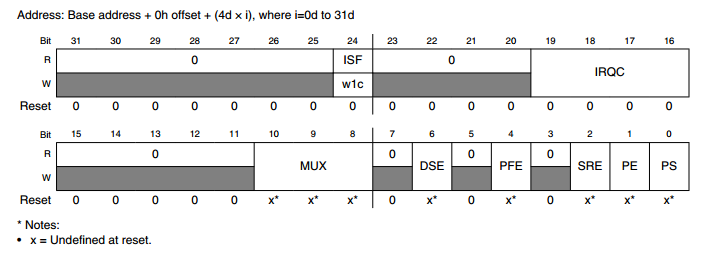
\includegraphics[width=100mm]{pcr.png}
\caption{Formatação do registrador PORTx\_PCR, onde pode-se ver os bits que configuram a função do pino (MUX)  \label{pcr}}
\end{figure}

Também é necessário configurar a direção dos pinos, pois este podem ser tanto Entrada (Input) como Saída (Output). Para isso, é preciso escrever no registrador \textbf{GPIOx\_PDDR} (\textbf{P}ort \textbf{D}ata \textbf{D}irection \textbf{R}egister) o valor ''1'' na posição correspondente do pino, seguindo a formatação mostrada na figura \ref{pddr}.

\begin{figure}[ht!]
\centering
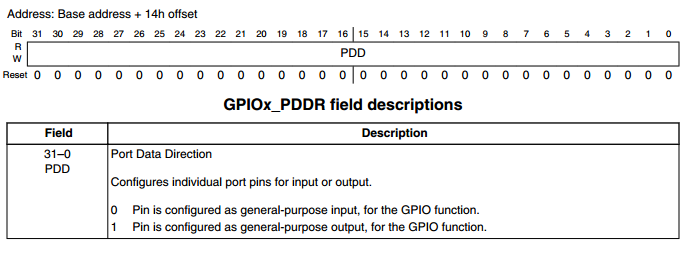
\includegraphics[width=100mm]{pddr.png}
\caption{Formatação do registrador GPIOx\_PDDR, mostrando a configuração da direção de cada pino GPIO  \label{pddr}}
\end{figure}

Para facilitar o reuso deste código de inicialização, foi criada uma função genérica que inicializa um pino por vez do LED RGB, recebendo então um valor inteiro e traduzindo-o em uma tabela da verdade para identificar os registradores que serão acessados.

Também foi criada uma função que inicializa todos os 3 pinos do LED RGB, sendo apenas um encapsulamento da função de incialização citada anteriormente dentro de um laço.

\subsubsection{Pseudo-código}

Um possível pseudo-código para a rotina de inicialização dos pinos do LED RGB é a mostrada a seguir.

\begin{verbatim}
INICIO (inicializa_led)
    Entrada: cor - Identificador (número inteiro) da cor do LED
    Saída: Pino do LED inicializado

    CASO cor
    vermelho:
        Seta em 1 o bit 10 do registrador SIM_SCGC5
        Seta em 1 o bit 8 do registrador PORTB_PCR18
        Seta em 0 os bits 9 e 10 do registrador PORTB_PCR18
        Seta em 1 o bit 18 do registrador GPIOB_PDDR
    verde:
        Seta em 1 o bit 10 do registrador SIM_SCGC5
        Seta em 1 o bit 8 do registrador PORTB_PCR19
        Seta em 0 os bits 9 e 10 do registrador PORTB_PCR19
        Seta em 1 o bit 19 do registrador GPIOB_PDDR
    azul:
        Seta em 1 o bit 12 do registrador SIM_SCGC5
        Seta em 1 o bit 8 do registrador PORTD_PCR1
        Seta em 0 os bits 9 e 10 do registrador PORTD_PCR1
        Seta em 1 o bit 1 do registrador GPIOD_PDDR
    FIM CASO
FIM
\end{verbatim}

Temos também o pseudo-código da função que inicializa todos os pinos do LED RGB:
\begin{verbatim}
INICIO (inicializa_led_rgb)
    Entrada: Nada
    Saída: Todos os pino do LED RGB inicializados

    PARA( cor MENOR QUE 3 )
        CHAMA incializa_led COM cor
        INCREMENTA cor
    FIM PARA
FIM
\end{verbatim}


\subsection{Atuação no LED}
Para atuar no LED RGB, ou seja, fazê-lo piscar precisamos escrever em registradores específicos que controlam o estado dos GPIOs.

Neste caso temos 3 registradores diferentes para cada porta GPIO:
\begin{itemize}
\item \textbf{GPIOx\_PSOR} (\textbf{P}ort \textbf{S}et \textbf{O}utput \textbf{R}egister) mostrado na figura \ref{psor}, usado para colocar o pino selecionado em nível alto (''1''), ou seja, apagar o LED
  \begin{figure}[ht!]
    \centering
    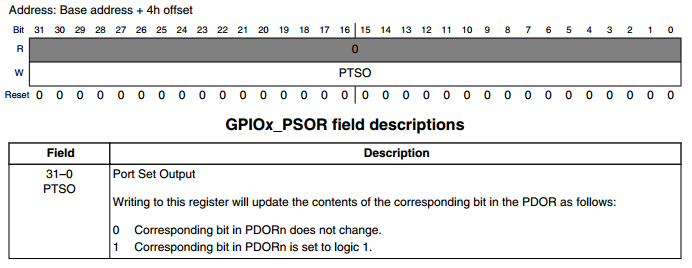
\includegraphics[width=100mm]{psor.png}
    \caption{Formatação do registrador GPIOx\_PSOR \label{psor}}
  \end{figure}

\item \textbf{GPIOx\_PCOR} (\textbf{P}ort \textbf{C}lear \textbf{O}utput \textbf{R}egister) mostrado na figura \ref{pcor}, usado para colocar o pino selecionado em nível baixo (''0''), ou seja, acender o LED
  \begin{figure}[ht!]
    \centering
    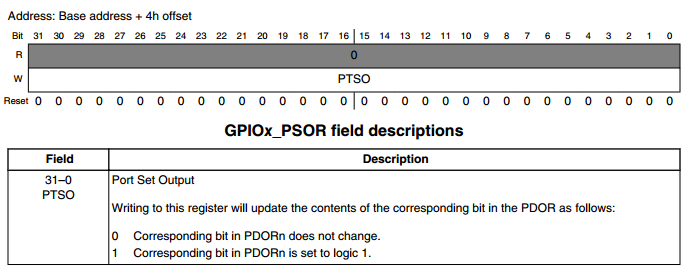
\includegraphics[width=100mm]{pcor.png}
    \caption{Formatação do registrador GPIOx\_PCOR \label{pcor}}
  \end{figure}

\item \textbf{GPIOx\_PTOR} (\textbf{P}ort \textbf{T}oggle \textbf{O}utput \textbf{R}egister) mostrado na figura \ref{ptor}, usado para inverter o estado lógico do pino selecionado
  \begin{figure}[ht!]
    \centering
    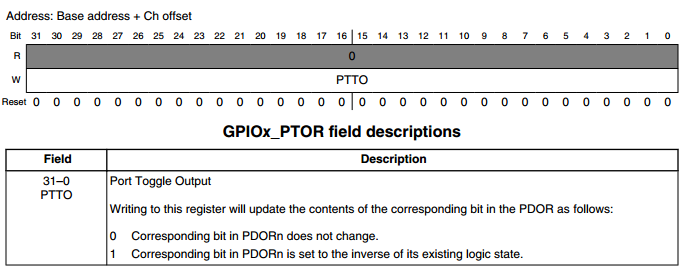
\includegraphics[width=100mm]{ptor.png}
    \caption{Formatação do registrador GPIOx\_PTOR \label{ptor}}
  \end{figure}
\end{itemize}

Novamente, para poder utilizar este módulo que controla o LED RGB no futuro, podem ser criadas 3 funções distintas: acender o LED, apagá-lo e inverter seu estado.

\subsubsection{Pseudo-código}

O Pseudo-código para a função que acende o LED pode ser escrito como a seguir. Vale lembrar que os registradores especificos e os pinos respectivos ao LED RGB serão definidos em uma estrutura separada no código em C.

\begin{itemize}
\item Função para acender o LED:
\begin{verbatim}
INICIO (acende_led)
    Entrada: Identificador (número inteiro) da cor do LED
    Saída: Pino do LED em estado lógico baixo ("0")

    Seta em 1 o bit correspondente ao pino do LED no registrador GPIOx_PCOR
FIM
\end{verbatim}

\item Função para apagar o LED:
\begin{verbatim}
INICIO (apaga_led)
    Entrada: Identificador (número inteiro) da cor do LED
    Saída: Pino do LED em estado lógico alto ("1")

    Seta em 1 o bit correspondente ao pino do LED no registrador GPIOx_PSOR
FIM
\end{verbatim}

\item Função para inverter o LED:
\begin{verbatim}
INICIO (inverte_led)
    Entrada: Identificador (número inteiro) da cor do LED
    Saída: Pino do LED em estado lógico alto invertido

    Seta em 1 o bit correspondente ao pino do LED no registrador GPIOx_PTOR
FIM
\end{verbatim}
\end{itemize}

\subsection{Atrasos}

Há várias formas de implementar rotinas de atraso em um ambiente embarcado. A mais simples e a que será explorada neste experimento é feita por um laço no qual uma variável é decrementada até 0, retornando desta rotina apenas no fim deste laço.

Neste experimento o número de iterações do laço decrementativo foi obtido empiricamente, mas é possível realizar o cálculo do tempo exato em que a rotina ficará em execução a partir do valor da frequência de clock do microcontrolador.

\subsubsection{Pseudo-código}

O Pseudo-código da função de atraso é como a seguir:

\begin{verbatim}
INICIO (Delay)
    Entrada: i - Número de iterações
    Saída: Nada

    ENQUANTO( i DIFERENTE DE 0 )
        DECREMENTA i
    FIM ENQUANTO
FIM
\end{verbatim}

\subsection{Laço principal - Main}

A função main contém o laço principal do programa e é chamada logo após a inicialização de baixo nível da memória.

Como todo o acesso aos registradores foi abstraído no módulo do LED RGB, a função main apenas faz chamadas às suas subrotinas.

\subsubsection{Pseudo-Código}
Um pseudo-código para a função main é o seguinte:

\begin{verbatim}
INICIO
    CHAMA inicializa_led_rgb
    ENQUANTO( verdadeiro )
        CHAMA inverte_led com 'vermelho'
        CHAMA inverte_led com 'verde'
        CHAMA inverte_led com 'azul'
        CHAMA delay com 500000
    FIM ENQUANTO
FIM
\end{verbatim}

\clearpage
\section{Testes}

Utilizando o IDE do CodeWarrior para realizar os testes, foi possível acompanhar a execução do programa passo-a-passo e resolver eventuais problemas de implementação do código em C.

\subsection{Registradores}
Uma das ferramentas do CodeWarrior utilizada para debug foi a aba ''Registers'', onde é possível ver e editar o valor em tempo real de todos os registradores do microcontrolador. Agrupando todos os que foram utilizados neste experimento, temos na figura \ref{reg_antes} seus valores antes da chamada da função de inicialização dos pinos do LED RGB. Já na figura \ref{reg_depois} vemos destacado em amarelo os valores alterados dos registradores de configuração (SIM\_SCGC5, PORTx\_PCRy e GPIOx\_PDDR).

\begin{figure}[ht!]
  \centering
  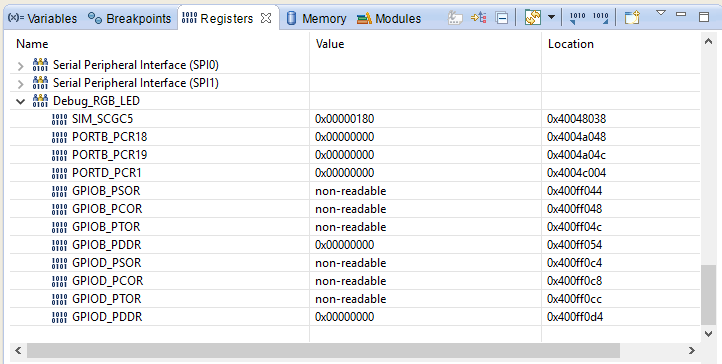
\includegraphics[width=160mm]{before_rgb_init.png}
  \caption{Estado dos registradores de configuração do LED RGB antes da chama da função de inicialização \label{reg_antes}}
\end{figure}

\begin{figure}[ht!]
  \centering
  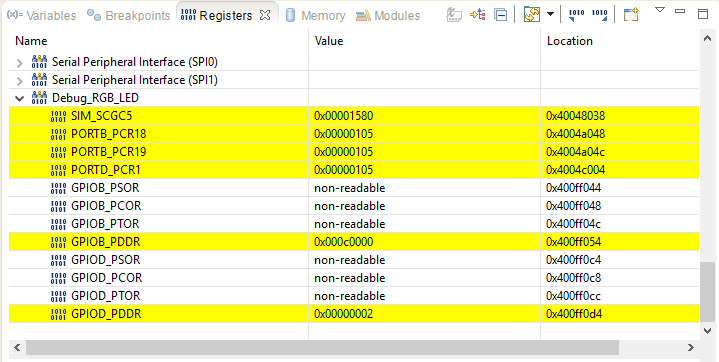
\includegraphics[width=160mm]{after_rgb_init.png}
  \caption{Estado dos registradores de configuração do LED RGB depois da chama da função de inicialização \label{reg_depois}}
\end{figure}

\subsection{Osciloscópio}

Também foi utilizado um osciloscópio comum para analisar a forma de onda gerada pelo pino do LED RGB.

Como o pino do Catodo Azul do LED (PTD1) está roteado na placa também para um conector externo (J2 - pino 12) foi possível medir a tensão neste ponto com a ponta de prova do osciloscópio, mostrada na figura \ref{wave_led}.

\begin{figure}[ht!]
  \centering
  \includegraphics[width=100mm]{wave_led.png}
  \caption{Forma de onda da tensão do pino 12 do conector J2 da placa FRDM-KL25Z que está ligado ao catodo azul do LED RGB \label{wave_led}}
\end{figure}

Na imagem do osciloscópio é possível ver também a medida do período da onda, que está relacionado diretamente ao valor inserido na função de atraso. No caso temos um período total de \SI{480}{\milli\second}, ou seja, o LED fica \SI{240}{\milli\second} ligado e o mesmo tempo desligado.

Como foi utilizada na implementação do programa a função de ''toggle'' do pino para termos um código mais enxuto, temos aqui um Duty Cycle de 50\% no LED.

\clearpage
\section{Conclusões}

A solução proposta para o experimento foi mais que suficiente para alcançar o objetivo final de piscar o LED RGB na cor branca. Tal atividade foi útil particulamente para embasar a criação de um módulo de controle para o LED RGB e de um módulo de funções de atraso que possam ser utilizados em futuros projetos da disciplina.

O módulo do LED RGB foi criado de modo a não serem precisos futuros desenvolvimentos, já que todas as funções necessárias a ele já foram implementadas (inicialização por cor ou de todo o led, acender, apagar e inverter), assim, ele está pronto para ser apenas incluido em outros projetos.

Um possível desenvolvimento do módulo de atraso consiste em relacionar o valor de Clock do relógio do microcontrolador com o número de iterações necessárias, ou seja, criar uma função que receba como argumento um valor de tempo e não de iterações.

O código foi todo documentado no estilo Doxygen \cite{doxygen} para que fosse possível gerar uma documentação em estilo profissional do projeto sem muito esforço.

Todos os código desenvolvidos nesta disciplina foram hospedados no repositório do aluno no GitHub \cite{github}.

\begin{thebibliography}{9} % Use for 1-9 references

\bibitem{code-warrior}
  Página inicial do CodeWarrior - Acessado em 21/03/2017\\
  \url{http://www.nxp.com/products/software-and-tools/software-development-tools/codewarrior-development-tools:CW_HOME}

\bibitem{manual-frdm}
  Manual da placa FRMD-KL25Z - Acessado em 21/03/2017\\
  \url{http://www.seeedstudio.com/document/pdf/FRMD-KL25Z.pdf}

\bibitem{manual-mic}
  Manual do microcontrolador Kinetis KL25Z128 - Acessado em 21/03/2017\\
  \url{http://cache.freescale.com/files/32bit/doc/ref_manual/KL25P80M48SF0RM.pdf}

\bibitem{github}
  Repositório do GitHub do aluno com os códigos da disciplina - Acessado em 21/03/2017\\
  \url{https://github.com/henrique-silva/ea871}

\bibitem{doxygen}
  Guia de documentação de código no estilo Doxygen - Acessado em 21/03/2017\\
  \url{https://www.stack.nl/~dimitri/doxygen/manual/docblocks.html}

\end{thebibliography}

\clearpage
\appendix
\section{Código Fonte - main.c}
\lstinputlisting[language=C]{/home/guife/rep/ea871/exp2/cw_project/Sources/main.c}

\clearpage
\section{Código Fonte - led\_rgb.c}
\lstinputlisting[language=C]{/home/guife/rep/ea871/exp2/cw_project/Sources/led_rgb.c}

\clearpage
\section{Código Fonte - led\_rgb.h}
\lstinputlisting[language=C]{/home/guife/rep/ea871/exp2/cw_project/Project_Headers/led_rgb.h}

\clearpage
\section{Código Fonte - delay.c}
\lstinputlisting[language=C]{/home/guife/rep/ea871/exp2/cw_project/Sources/delay.c}

\clearpage
\section{Código Fonte - delay.h}
\lstinputlisting[language=C]{/home/guife/rep/ea871/exp2/cw_project/Project_Headers/delay.h}
\end{document}
